\DocumentMetadata{
  pdfversion=2.0,
  pdfstandard=ua-2,
  testphase={phase-III,math,table,title}
}

\documentclass[10pt]{article}
\usepackage{geometry}
\geometry{a4paper}
\usepackage{fancyhdr}
\usepackage{lastpage}
\usepackage{extramarks}
\usepackage[usenames,dvipsnames]{color}
\usepackage{graphicx}
\usepackage{listings}
\usepackage{courier}
\usepackage{lipsum}
\usepackage{caption}
\usepackage{subcaption}
\usepackage{amsmath}
\usepackage{amssymb}
\usepackage{epstopdf}
\usepackage{placeins}
\usepackage{color} 
\usepackage{fancyvrb} 
\usepackage{setspace}
\usepackage{bookmark}
\usepackage{pdfpages}
\usepackage{enumitem}
\usepackage{tikz}
\usepackage{pgfplots}
\usepackage{hyperref}
\usepackage{circuitikz}
\usepackage{siunitx}
\usepackage{titling}

\DeclareGraphicsExtensions{.pdf,.png,.jpg}
\graphicspath{{../figs/}}

\usetikzlibrary{positioning}
\usetikzlibrary{calc}

\pgfplotsset{compat=newest} 

\setlength{\parindent}{0pt}

\singlespacing

% Margins
\topmargin=-0.45in
\evensidemargin=0in
\oddsidemargin=0in
\textwidth=6.5in
\textheight=9.0in
\headsep=0.25in

% Header and footer
\pagestyle{fancy}

% Ensure the plain style (used by \maketitle and some environments) matches
\fancypagestyle{plain}{
  \fancyhf{}
  \lhead{ECEN 222:   Electronic Circuits II-CE}
  \chead{Lab 9}
  \rhead{Page \thepage\ of \pageref{LastPage}}
  \lfoot{}
  \cfoot{}
  \rfoot{Maxx Seminario, mseminario2@huskers.unl.edu}
  \renewcommand\headrulewidth{0.4pt}
  \renewcommand\footrulewidth{0.4pt}
}

% Fancy layout (same as above) for normal pages
\fancyhf{}
\lhead{ECEN 222: Electronic Circuits II-CE}
\chead{Lab 9}
\rhead{Page \thepage\ of \pageref{LastPage}}
\lfoot{}
\cfoot{}
\rfoot{Maxx Seminario, mseminario2@huskers.unl. edu}
\renewcommand\headrulewidth{0.4pt}
\renewcommand\footrulewidth{0.4pt}

% Avoid head height warnings
\setlength{\headheight}{14pt}

\title{\textbf{\Huge Ring Oscillator Design and Clock Generation for Digital Systems}\\
\large Lab 9 — ECEN 222: Electronic Circuits II-CE}
\author{
\large University of Nebraska-Lincoln \\
\large Department of Electrical and Computer Engineering
}
\date{} % specific date

\begin{document}
\thispagestyle{fancy}
\maketitle
\rule{\textwidth}{0.5pt}

\section{Objectives}

The primary objective of this lab is to design, construct, and characterize a ring oscillator circuit using discrete logic gates as a practical introduction to digital integrated circuits and clock signal generation.  Upon completion of this lab, students will understand the fundamental principle of ring oscillator operation using an odd number of inverting stages, design and implement enable/disable control circuitry using NAND or NOR logic gates, measure and characterize oscillation frequency and duty cycle using oscilloscopes and frequency counters, investigate methods for frequency tuning including varying the number of inverter stages and adjusting gate propagation delays, analyze the relationship between gate propagation delay and oscillation frequency, understand parasitic capacitance and its effect on oscillator performance, recognize the practical application of ring oscillators as clock signal generators for sequential digital systems, and compare experimental measurements with theoretical predictions based on gate propagation delays and circuit topology.  Through hands-on construction and testing, students will bridge the gap between analog circuit analysis and digital system design, developing practical skills in timing analysis and clock generation essential for microprocessors, counters, shift registers, and other synchronous digital systems.

\section{Pre-Lab Preparation}

Before arriving at the lab session, students are required to thoroughly prepare by reading the relevant material from the course textbook and supplementary resources.  Specifically, review Chapter 14 (Digital Integrated Circuits) in Sedra \& Smith or equivalent digital electronics material, focusing on sections covering CMOS logic gates (inverters, NAND, NOR), propagation delay and timing parameters in digital circuits, the concept of feedback and oscillation in digital systems, and basic sequential logic and clocking requirements. If using TTL logic families, review TTL specifications including $V_{OH}$, $V_{OL}$, $V_{IH}$, $V_{IL}$, propagation delay ($t_{pd}$), and fan-out limitations. For CMOS logic families (74HC or 74HCT series), review CMOS characteristics including near rail-to-rail swing, input capacitance, and how RC time constants affect switching speed. Additionally, review oscilloscope operation for measuring frequency, period, duty cycle, and rise/fall times. Students must also complete the pre-lab questions provided in Section \ref{sec:prelab}, which include preliminary calculations for oscillator frequency based on assumed gate delays.  Bring these calculations to lab—they will guide your initial circuit design and help you select appropriate component values.  Proper preparation will ensure efficient use of lab time and enable meaningful comparison between theoretical predictions and experimental results.  Familiarize yourself with the datasheet for the specific logic IC family you will be using in lab (e.g., 74HC04 hex inverter, 74HC00 quad NAND gate).

\section{Background Theory}

\subsection{Ring Oscillator Fundamentals}

A ring oscillator is one of the simplest oscillator circuits, consisting of an odd number of inverting stages connected in a closed loop (ring). The fundamental principle relies on the fact that any signal propagating through the loop will be inverted an odd number of times, creating inherent instability that results in continuous oscillation. 

\subsubsection{Basic Operation Principle}

Consider a simple three-inverter ring oscillator. If we assume the output of the first inverter is initially HIGH: 

\begin{enumerate}
    \item The first inverter outputs HIGH
    \item After propagation delay $t_{pd1}$, the second inverter receives HIGH and outputs LOW
    \item After propagation delay $t_{pd2}$, the third inverter receives LOW and outputs HIGH
    \item After propagation delay $t_{pd3}$, the first inverter receives HIGH and outputs LOW
    \item The cycle repeats with inverted logic levels
\end{enumerate}

The key insight is that the output of the final stage is fed back to the input of the first stage, and because there are an odd number of inversions (three), the feedback is negative at DC but creates a timing condition that sustains oscillation.

\subsubsection{Oscillation Frequency Calculation}

For a ring oscillator with $N$ inverting stages (where $N$ must be odd), each with propagation delay $t_{pd}$, the signal must propagate through all $N$ stages to complete one half-cycle of oscillation. Therefore, the period is:

\begin{equation}
    T = 2 \times N \times t_{pd}
    \label{eq:period}
\end{equation}

The factor of 2 accounts for the fact that the signal must traverse the entire ring twice (once for HIGH-to-LOW transitions, once for LOW-to-HIGH transitions) to return to its original state.

The oscillation frequency is: 

\begin{equation}
    f_{osc} = \frac{1}{T} = \frac{1}{2 N t_{pd}}
    \label{eq:frequency}
\end{equation}

This equation reveals several important design considerations:

\begin{itemize}
    \item Increasing the number of stages $N$ decreases the oscillation frequency
    \item Gates with faster propagation delays produce higher frequency oscillations
    \item For a given gate type, frequency can be tuned by changing $N$
\end{itemize}

\subsubsection{Propagation Delay in Logic Gates}

The propagation delay $t_{pd}$ is the time required for a logic gate's output to respond to a change in its input. It is typically defined as the time between the 50\% point of the input transition and the 50\% point of the corresponding output transition.

For CMOS logic gates, the propagation delay depends on several factors:

\begin{equation}
    t_{pd} \approx \frac{C_L \Delta V}{I_{avg}}
    \label{eq:prop_delay}
\end{equation}

where:
\begin{itemize}
    \item $C_L$ is the load capacitance (including gate input capacitance and parasitic capacitance)
    \item $\Delta V$ is the voltage swing (typically $V_{DD}$ for rail-to-rail CMOS)
    \item $I_{avg}$ is the average current available to charge/discharge the capacitance
\end{itemize}

This relationship shows that propagation delay increases with load capacitance.  This fact can be exploited to tune oscillator frequency by adding external capacitance. 


\subsection{Enable/Disable Control Using Logic Gates}

For practical applications, it is essential to be able to start and stop the oscillator.  Simply breaking the ring would work, but a more elegant solution uses a control gate that can conditionally enable or disable the feedback path. 

\subsubsection{NAND Gate Enable Circuit}

A common implementation uses a two-input NAND gate as one of the stages in the ring, with one input serving as the oscillator output feedback and the other as an active-HIGH enable signal. 

\begin{figure}[h]
\centering
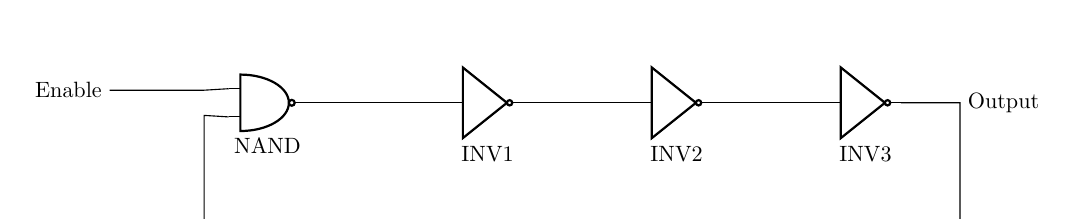
\begin{tikzpicture}[scale=0.8, every node/.style={scale=0.8}]
    % Define logic gate style
    \tikzstyle{gate} = [draw, minimum size=1cm]
    
    % NAND gate with enable
    \node[nand port, scale=0.8] (nand1) at (0,0) {};
    
    % Inverters
    \node[not port, scale=0.8] (inv1) at (3,0) {};
    \node[not port, scale=0.8] (inv2) at (6,0) {};
    \node[not port, scale=0.8] (inv3) at (9,0) {};
    
    % Connections - forward path
    \draw (nand1.out) -- (inv1.in);
    \draw (inv1.out) -- (inv2.in);
    \draw (inv2.out) -- (inv3.in);
    
    % Feedback path
    \draw (inv3.out) -- (10.5,0) -- (10.5,-2) -- (-1.5,-2) -- (-1.5,-0.2) -- (nand1.in 2);
    
    % Enable input
    \draw (nand1.in 1) -- (-1.5,0.2) -- (-3,0.2) node[left] {Enable};
    
    % Output
    \draw (inv3.out) -- (10.5,0) node[right] {Output};
    
    % Node labels
    \node[below] at (nand1.south) {NAND};
    \node[below] at (inv1.south) {INV1};
    \node[below] at (inv2.south) {INV2};
    \node[below] at (inv3.south) {INV3};
    
\end{tikzpicture}
\caption{Ring oscillator with NAND gate enable control (4 stages, 4 inversions).}
\label{fig:ring_nand}
\end{figure}

Operation: 
\begin{itemize}
    \item When Enable = HIGH (logic 1), the NAND gate acts as an inverter for the feedback signal, and the ring oscillates (4 stages, 4 inversions total = even, so this won't oscillate)
    \item When Enable = LOW (logic 0), the NAND output is forced HIGH regardless of feedback, breaking oscillation
\end{itemize}

\textbf{Important: } The total number of inversions in the loop must be odd.  A NAND gate with one input HIGH acts as an inverter.  In the configuration shown in Figure \ref{fig:ring_nand}, there are 4 inversions (NAND + 3 inverters), which is even—this will NOT oscillate.  To fix this, we need either:
\begin{itemize}
    \item Create an odd number of total stages (NAND + even number of inverters), or
    \item Replace one inverter with a buffer (non-inverting)
\end{itemize}

\subsubsection{NOR Gate Enable Circuit}

Alternatively, a NOR gate can be used with active-LOW enable control: 

\begin{figure}[h]
\centering
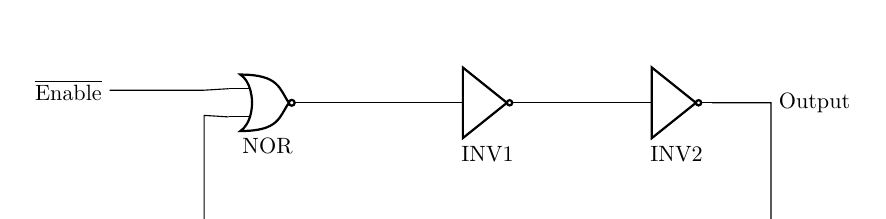
\begin{tikzpicture}[scale=0.8, every node/.style={scale=0.8}]
    % NOR gate with enable
    \node[nor port, scale=0.8] (nor1) at (0,0) {};
    
    % Inverters  
    \node[not port, scale=0.8] (inv1) at (3,0) {};
    \node[not port, scale=0.8] (inv2) at (6,0) {};
    
    % Connections - forward path
    \draw (nor1.out) -- (inv1.in);
    \draw (inv1.out) -- (inv2.in);
    
    % Feedback path
    \draw (inv2.out) -- (7.5,0) -- (7.5,-2) -- (-1.5,-2) -- (-1.5,-0.2) -- (nor1.in 2);
    
    % Enable input (active LOW)
    \draw (nor1.in 1) -- (-1.5,0.2) -- (-3,0.2) node[left] {$\overline{\text{Enable}}$};
    
    % Output
    \draw (inv2.out) -- (7.5,0) node[right] {Output};
    
    % Node labels
    \node[below] at (nor1.south) {NOR};
    \node[below] at (inv1.south) {INV1};
    \node[below] at (inv2.south) {INV2};
    
\end{tikzpicture}
\caption{Ring oscillator with NOR gate enable control (3 stages, 3 inversions).}
\label{fig:ring_nor}
\end{figure}

Operation:
\begin{itemize}
    \item When $\overline{\text{Enable}}$ = LOW (logic 0), the NOR gate acts as an inverter for the feedback signal, and the ring oscillates (3 inversions total)
    \item When $\overline{\text{Enable}}$ = HIGH (logic 1), the NOR output is forced LOW, breaking oscillation
\end{itemize}

This configuration has 3 total inversions (odd), so it will oscillate when enabled.

\subsection{Frequency Tuning Methods}

There are several practical methods to adjust the oscillation frequency of a ring oscillator:

\subsubsection{Method 1: Varying the Number of Inverter Stages}

From Equation \ref{eq:frequency}, increasing $N$ decreases frequency.  This is the most straightforward tuning method.\\

Advantages:
\begin{itemize}
    \item Discrete, predictable frequency steps
    \item No additional components required
    \item Frequency ratios are precise (inversely proportional to $N$)
\end{itemize}

Disadvantages: 
\begin{itemize}
    \item Requires circuit modification (adding/removing gates)
    \item Cannot be adjusted in real-time
    \item Limited to discrete values
\end{itemize}

\subsubsection{Method 2: Adding External Capacitance}

By adding small capacitors from each inverter output to ground, the propagation delay increases according to Equation \ref{eq:prop_delay}. The effective propagation delay becomes:

\begin{equation}
    t_{pd,eff} = t_{pd,intrinsic} + \frac{C_{ext} \Delta V}{I_{avg}}
    \label{eq:prop_delay_ext}
\end{equation}

where $C_{ext}$ is the external added capacitance. \\

For a variable capacitor (varactor diode or tuning capacitor), continuous frequency adjustment is possible: 

\begin{equation}
    f_{osc} = \frac{1}{2N(t_{pd,intrinsic} + k \cdot C_{ext})}
    \label{eq:freq_tuned}
\end{equation}

where $k = \Delta V / I_{avg}$ is a constant depending on the gate characteristics. \\

Advantages:
\begin{itemize}
    \item Continuous frequency tuning
    \item Can be implemented with potentiometer for manual tuning
    \item Can be voltage-controlled with varactor diodes
\end{itemize}

Disadvantages: 
\begin{itemize}
    \item Tuning range is limited (typically 2:1 to 3:1 ratio)
    \item Requires additional components
    \item May affect signal quality (slower edges, reduced noise margin)
    \item Non-linear relationship between capacitance and frequency
\end{itemize}


\subsection{Applications in Digital Systems}

Ring oscillators serve as clock signal generators for various digital applications:

\subsubsection{Sequential Digital Systems}

Sequential logic circuits—including flip-flops, counters, shift registers, and state machines—require a clock signal to synchronize state transitions. The clock must meet specific requirements:

\begin{itemize}
    \item \textbf{Frequency stability: } The clock frequency should remain constant over time and temperature
    \item \textbf{Duty cycle:} The ratio of HIGH time to total period, ideally 50\% for symmetric operation
    \item \textbf{Edge quality:} Fast rise and fall times ensure well-defined triggering moments
    \item \textbf{Jitter:} Cycle-to-cycle period variation should be minimized
\end{itemize}

Ring oscillators provide adequate performance for many educational and low-cost applications, though crystal oscillators offer superior stability for precision timing. 

\subsubsection{Microprocessor and Microcontroller Clocking}

Modern microprocessors require high-frequency, stable clocks. While production systems use crystal oscillators and phase-locked loops (PLLs), ring oscillators are commonly used: 

\begin{itemize}
    \item As on-chip RC oscillators for initial boot-up before external crystal stabilizes
    \item In low-power sleep modes where precision is not critical
    \item For watchdog timers and timeout functions
    \item In PLLs as voltage-controlled oscillators (VCOs)
\end{itemize}

\subsubsection{PWM and Timing Generation}

Ring oscillators can generate timing references for: 
\begin{itemize}
    \item Pulse-width modulation (PWM) circuits
    \item Delay lines and timing circuits
    \item Baud rate generators for serial communication
    \item Sampling clocks for analog-to-digital converters (ADCs)
\end{itemize}


Ideally, a ring oscillator with symmetric inverters produces a 50\% duty cycle. However, asymmetry in rise and fall times ($t_{pLH} \neq t_{pHL}$) causes duty cycle deviation:

\begin{equation}
    \text{Duty Cycle} = \frac{N \cdot t_{pLH}}{N \cdot t_{pLH} + N \cdot t_{pHL}} = \frac{t_{pLH}}{t_{pLH} + t_{pHL}}
\end{equation}

For CMOS logic with similar PMOS and NMOS strengths, duty cycles are typically 45-55\%. 

\section{Experimental Procedures}

\subsection{Part 1: Basic 3-Stage Ring Oscillator}

In this first part, you will construct the simplest possible ring oscillator using three inverters and observe its basic operation.

\subsubsection{Circuit Construction}

\begin{enumerate}
    \item Obtain a few CMOS inverters. Check the datasheet for pinout and propagation delay specifications.
    
    \item Add a 0.1 µF ceramic decoupling capacitor between $V_{DD}$ and GND, placed as close as possible to the IC. 
    
    \item Connect three inverters in a ring. Be sure to refer to the IC pinout diagram to identify individual inverter inputs and outputs.
    
    \item Before applying power, visually verify the connections.  Ensure you have an odd number of inverting stages in the loop.
\end{enumerate}

\subsubsection{Initial Testing and Measurement}

\begin{enumerate}
    \item Apply power to the circuit.  The oscillator should start immediately.
    
    \item Connect an oscilloscope probe to the output any inverter. Use a ground clip connection to minimize noise.
    
    \item Observe the waveform.  You should see a square or sine wave oscillation.  Adjust timebase to show 3-5 complete cycles.
    
    \item Measure and record:
    \begin{itemize}
        \item Period $T$ (time for one complete cycle)
        \item Frequency $f = 1/T$
        \item Peak-to-peak voltage (should be approximately $V_{DD}$)
        \item Duty cycle (percentage of time the signal is HIGH)
    \end{itemize}
    
    \item Capture an oscilloscope screenshot showing several complete cycles with cursors measuring the period. 
\end{enumerate}

\subsubsection{Analysis and Comparison}

\begin{enumerate}
    \item From the datasheet, find the typical propagation delay $t_{pd}$ for your inverter IC at $V_{DD} = 5$ V with the specified load capacitance.
    
    \item Calculate the theoretical oscillation frequency using Equation \ref{eq:frequency} with $N = 3$:
    \begin{equation}
        f_{theoretical} = \frac{1}{2 \times 3 \times t_{pd}} = \frac{1}{6 t_{pd}}
    \end{equation}
    
    \item Compare measured vs. theoretical frequency. Calculate percentage error.
    
    \item Discuss sources of discrepancy.
    
    \item Measure the rise time and fall time of the output waveform (10\% to 90\% transition times). These should be much faster than the propagation delay. 
\end{enumerate}

\subsection{Part 2: Ring Oscillator with Enable Control}

Now you will add enable/disable functionality using a NAND gate, creating a practical controllable oscillator.

\subsubsection{Circuit Design}

Choose one of two implementations: \\

\textbf{Option A:  NAND-based enable (active HIGH)}
\begin{enumerate}
    \item Obtain CMOS Inverter ICs and a 2-input NAND gate IC. 
    \item Replace one inverter in your 3-stage ring with a NAND gate
    \item This creates only 2 inversions (1 NAND + 1 inverter), which is even—won't oscillate.
    \item Add two more inverters to make 5 total stages (1 NAND + 4 inverters = 5 inversions, odd)
    \item Connect one NAND input to the feedback path
    \item Connect the other NAND input to a control switch (pulled HIGH to enable, LOW to disable)
\end{enumerate}

\textbf{Option B: NOR-based enable (active LOW)}
\begin{enumerate}
    \item Obtain CMOS Inverter ICs and a 2-input NAND gate IC. 
    \item Replace one inverter with a NOR gate
    \item Use 3 total stages:  1 NOR + 2 inverters (3 inversions, odd)
    \item Connect one NOR input to the feedback path
    \item Connect the other NOR input to a control switch (pulled LOW to enable, HIGH to disable)
\end{enumerate}

\subsubsection{Control Switch Implementation}

Implement the enable control using a switch or button:

\begin{enumerate}
    \item For NAND gate (active HIGH enable):
    \begin{itemize}
        \item Connect enable input through a 10 k$\Omega$ pull-down resistor to ground
        \item Connect switch from enable input to $V_{DD}$
        \item Switch closed = HIGH = oscillator enabled
        \item Switch open = LOW = oscillator disabled
    \end{itemize}
    
\end{enumerate}

\subsubsection{Testing Enable Functionality}

\begin{enumerate}
    \item With oscilloscope connected to the output, toggle the enable switch. 
    
    \item Verify that: 
    \begin{itemize}
        \item When enabled, oscillation occurs
        \item When disabled, output remains at a constant logic level
    \end{itemize}
    
    \item Measure the oscillation frequency when enabled.  It should be lower than the 3-stage oscillator due to the increased number of stages.
    
    \item Calculate the expected frequency based on the number of stages and compare with measurement.
    
    \item Observe what happens immediately after enabling: 
    \begin{itemize}
        \item Does oscillation start instantly?
        \item What is the initial transient behavior?
    \end{itemize}
    
    \item Capture oscilloscope screenshots showing: 
    \begin{itemize}
        \item Oscillation when enabled
        \item Oscillation disabled (steady output)
        \item Transition from disabled to enabled (trigger on enable signal)
    \end{itemize}
\end{enumerate}

\subsection{Part 3: Frequency Tuning by Varying Inverter Stages}

In this part, you will experimentally investigate how the number of inverter stages affects oscillation frequency.

\subsubsection{Multi-Stage Configurations}

Build and test ring oscillators with different numbers of stages.  For each configuration, maintain the enable control gate and vary only the number of additional inverters. \\

Test the following configurations:
\begin{enumerate}
    \item 3 stages total (1 control gate + 2 inverters)
    \item 5 stages total (1 control gate + 4 inverters)
    \item 7 stages total (1 control gate + 6 inverters)
    \item 9 stages total (1 control gate + 8 inverters)
\end{enumerate}

\subsubsection{Measurements}

For each configuration: 
\begin{enumerate}
    \item Construct the circuit.
    
    \item Enable the oscillator and measure: 
    \begin{itemize}
        \item Frequency 
        \item Period
        \item Duty cycle
    \end{itemize}
    
    \item Calculate theoretical frequency using $f = 1/(2Nt_{pd})$
    
    \item Record all measurements in a table
\end{enumerate}

\subsubsection{Analysis}

\begin{enumerate}
    \item Create a table with columns: $N$ (number of stages), $f_{theoretical}$, $f_{measured}$, percentage error. 
    
    \item Plot measured frequency vs. number of stages. Use both: 
    \begin{itemize}
        \item Linear scale plot
        \item Plot of $1/f$ vs. $N$ 
    \end{itemize}
    
    \item From the $1/f$ vs. $N$ plot, perform linear regression.  The slope gives $2t_{pd}$.  Calculate the effective propagation delay from your measurements.
    
    \item Compare the extracted $t_{pd}$ with the datasheet value.  Discuss agreement and sources of deviation.
    
    \item Determine the practical frequency range achievable with your IC family using 3 to 11 stages.
\end{enumerate}


\subsection{Part 5: Application - Clock Signal for a Counter}

Demonstrate the practical application of your ring oscillator as a clock generator for a sequential digital circuit.

\subsubsection{Counter Circuit Construction}

\begin{enumerate}
    \item Obtain a binary counter IC.
    
    \item Build your 5-stage ring oscillator with enable control from Part 2.
    
    \item Connect the oscillator output to the clock input of the counter IC.
    
    \item Connect the counter outputs (Q0, Q1, Q2, Q3) to LEDs through current-limiting resistors.
    
    \item Add a reset button to manually reset the counter to zero.
\end{enumerate}

\subsubsection{Operation and Observation}

\begin{enumerate}
    
    \item Enable and Disable the oscillator and observe the number of oscillations on the LEDs in binary. 
    
    \item Use the oscilloscope to simultaneously display: 
    \begin{itemize}
        \item Clock signal (oscillator output)
        \item One of the counter outputs (e.g., Q0 or Q1)
    \end{itemize}
    
    \item Verify the relationship:  Q0 toggles at half the clock frequency.
    
    \item Test the enable control:  disabling the oscillator should stop the count.
    
    \item Demonstrate that the system functions as a basic sequential digital system with your ring oscillator providing the timing reference.
\end{enumerate}

\subsubsection{Analysis}

\begin{enumerate}
    \item Calculate the counting rate (increments per second) from the oscillator frequency.
    
    \item Verify that the observed counting rate matches the calculation. 
    
    \item Discuss the advantages and disadvantages of ring oscillators for clock generation: 
    
    \item Research and compare with alternative clock sources (crystal oscillators, RC oscillators, ceramic resonators) in terms of accuracy, stability, cost, and complexity.
\end{enumerate}

\section{Pre-Lab Questions}
\label{sec:prelab}

Complete these questions before coming to the lab session.  Include your answers and all supporting work in your lab report.

\begin{enumerate}
    
    \item \textbf{Propagation delay and frequency calculation:}
    \begin{enumerate}
        \item Look up the datasheet for the IC inverter you will use in this lab. Find the typical propagation delay ($t_{pd}$ or $t_{pLH}$ and $t_{pHL}$) at $V_{DD} = 5$ V with a 15 pF load capacitance.
        \item Calculate the theoretical oscillation frequency for a 3-stage ring oscillator using this propagation delay.
        \item Calculate the theoretical frequencies for 5-stage, 7-stage, and 9-stage configurations.
        \item Create a table summarizing your results.
    \end{enumerate}
    
    \item \textbf{Odd vs. even inversions:}
    \begin{enumerate}
        \item Explain in your own words why a ring oscillator requires an odd number of inverting stages.
        \item What would happen if you connected an even number of inverters in a ring? Describe the steady-state behavior.
        \item Draw a timing diagram (logic levels vs. time) for a 3-stage ring oscillator showing how the signal propagates through all three stages over two complete cycles.
    \end{enumerate}
    
    \item \textbf{Frequency tuning analysis:}
    \begin{enumerate}
        \item A ring oscillator with 5 stages oscillates at 10 MHz. What frequency would you expect if you increased it to 7 stages (assuming identical gate delays)?
        \item If you add a 50 pF capacitor to one stage output, increasing that stage's propagation delay from 10 ns to 15 ns, calculate the new oscillation frequency for the 5-stage oscillator.
    \end{enumerate}
    
\end{enumerate}


\end{document}